\documentclass[11pt]{report}
\usepackage{textcomp}

\usepackage{titlesec}
\titlespacing*{\section}
{0pt}{\baselineskip}{0em}
\titlespacing*{\subsection}
{0pt}{\baselineskip}{0em}

\usepackage{geometry}
\geometry{left=1in, right=1in, top=1in, textheight=9in}

\usepackage{enumitem}
\newlist{steps}{enumerate}{1}
\setlist[steps, 1]{wide=0pt, leftmargin=\parindent, label=Step \arabic*:}

\usepackage{fancyhdr}
\fancypagestyle{plain}{%
    \fancyhf{} % clear all header and footer fields
    \fancyfoot[C]{\sffamily\fontsize{.75em}{.75em}\selectfont\thepage} % except the center
    \renewcommand{\headrulewidth}{0pt}
    \renewcommand{\footrulewidth}{0pt}
}
\pagestyle{plain}

\usepackage{graphicx}
\graphicspath{ {./media/} }

\usepackage{setspace}
\doublespacing

\usepackage{minted}
\usepackage{xcolor}
\definecolor{LightGray}{gray}{0.9}
\newmintinline[asm]{asm}{fontsize=\small, bgcolor=LightGray}
\newmintinline[cpp]{cpp}{fontsize=\small, bgcolor=LightGray}

% make fancy title page
\makeatletter
\newcommand{\@labsection}{000}
\newcommand{\labsection}[1]{
    \renewcommand{\@labsection}{#1}
}

\newcommand{\@labnumber}{0}
\newcommand{\labnumber}[1]{
    \renewcommand{\@labnumber}{#1}
}

\newcommand{\@shortsubmitted}{1/1/70}
\newcommand{\shortsubmitted}[1]{
    \renewcommand{\@shortsubmitted}{#1}
}

\lfoot{\footnotesize \textit{University of Arkansas \\ EECS Department}}
\rfoot{\footnotesize \textsl{\@shortsubmitted}}

\renewcommand{\maketitle}{
    \newgeometry{left=1in, right=1in, top=1.75in, textheight=8.25in}
    \singlespacing
    \begin{center}
        {\huge \bf CSCE 22104} \\
        \vspace{2.5em}
        {\Large \bf Lab Report} \\
        \vspace{2em}
        \noindent\rule{20em}{0.4pt} \\
        \vspace{1em}
        {\Large \@author} \\
        \vspace{.75em}
        {\normalsize ID: 011019116} \\
        \vspace{.75em}
        {\normalsize Lab Section \@labsection} \\
        \vspace{.75em}
        {\normalsize Lab \@labnumber} \\
    \end{center}
    \newpage
    \restoregeometry
}

\makeatother


% TEXTWIDTH = 100
\begin{document}
\title{Lab Report 4}
\author{Brent Marcus Orlina}

\labsection{001}
\labnumber{4}

\shortsubmitted{2/5/25}

\maketitle

\section*{Introduction}
This lab's goal was to create and call a function, \verb|compare_and_swap|, in MIPS that is used by
a bubble sort algorithm provided. The function is provided with two memory addresses in the
registers \verb|$a0| and \verb|$a1|. If the value in the memory address \verb|$a1| is less than the
value in the memory address \verb|$a0|, then the values should be swapped. In other words, the lesser
value should live in \verb|$a0| and the greater the value should live in \verb|$a1|.

To correctly call the function for the bubble sort algorithm, the addresses of the element of a
given index and the element after it is stored in the registers \verb|$a0| and \verb|$a1|. The given
index has already been provided in the bubble sort algorithm. Then, the function is called using the
jump-and-link instruction, \verb|jal|. 

\section*{Approach}
\begin{listing}[h!]
    \inputminted[
        frame=lines,
        breaklines,
        linenos,
        tabsize=4,
        fontsize=\footnotesize,
        bgcolor=LightGray
    ]{asm}{./media/compare_and_swap.s}
    \caption{Implementation of the \texttt{compare\_and\_swap} function in MIPS.}
    \label{listing:compare_and_swap}
\end{listing}

The function \verb|compare_and_swap| in listing \ref{listing:compare_and_swap} is called with the
addresses of the elements to be compared and swapped in registers \verb|$a0| and \verb|$a1|. The
contents in the two addresses is loaded into two registers \verb|$t0| and \verb|$t1| respectively.
The values are then compared with the branch instruction \verb|ble|. That is, if the value in
\verb|$t0| is already less than or equal to the value in \verb|$t1|, there is no need to swap and
jumps to \verb|compare_and_swap_exit|. Otherwise, the value in \verb|$t0| is greater than in
\verb|$t1| which means that the two elements must be swapped. The swap occurs in line 5 and 6. The
value in \verb|$t1| is stored into the memory address in \verb|$a0| and the value in \verb|$t0| is
stored into the memory address in \verb|$a1|. In \verb|compare_and_swap_exit|, it returns to the
caller by jumping to the return address in \verb|$ra|.

\begin{listing}[!ht]
    \inputminted[
        frame=lines,
        breaklines,
        linenos,
        tabsize=4,
        fontsize=\footnotesize,
        bgcolor=LightGray
    ]{cpp}{./media/bubble_sort.cpp}
    \caption{The bubble sort algorithm.}
    \label{listing:bubble_sort}
\end{listing}

\begin{listing}[!ht]
    \inputminted[
        frame=lines,
        breaklines,
        linenos,
        tabsize=4,
        fontsize=\footnotesize,
        bgcolor=LightGray
    ]{asm}{./media/compare_and_swap_call.s}
\caption{Implementation of the call to the \texttt{compare\_and\_swap} function in MIPS.}
    \label{listing:compare_and_swap_call}
\end{listing}

Listing \ref{listing:bubble_sort} shows the bubble sort algorithm. Translation from C++ to MIPS of
lines 1 to 3 were provided, leaving the call to \verb|compare_and_swap| to be implemented. In
listing \ref{listing:compare_and_swap_call}, the base address of the array is stored in register
\verb|$s0| and the inner-loop index, \verb|j| is stored in register \verb|$s3|. The arrays store an
\verb|int| which have a size of 4 bytes. Therefore, we must multiply the inner-loop index by 4 to
achieve the correct offset. Line 2 of listing \ref{listing:compare_and_swap_call} achieves the same
goal by left shifting by 2. Then, the address \cpp{&(arr[j])} is calculated by adding the base
address of the array with the offset, which is stored into the first argument register, \verb|$a0|.
The address \cpp{&(arr[j + 1])} is calculated by adding 4 to the previously calculated address,
which is stored into the second argument register, \verb|$a1|. Now that the arguments have been
provided for the \verb|compare_and_swap| function, it is finally called with the \verb|jal|
instruction.

\section*{Experimentation}
The bubble sort algorithm, therefore the function \verb|compare_and_swap| implementation as well,
was tested by sorting an array containing random integers in random order and an array of powers of
two in decreasing order. The bubble sort algorithm worked as expected and sorted each array in
increasing order.

\newpage

\section*{Results \& Discussion}
\begin{figure}[h!]
    \centering
    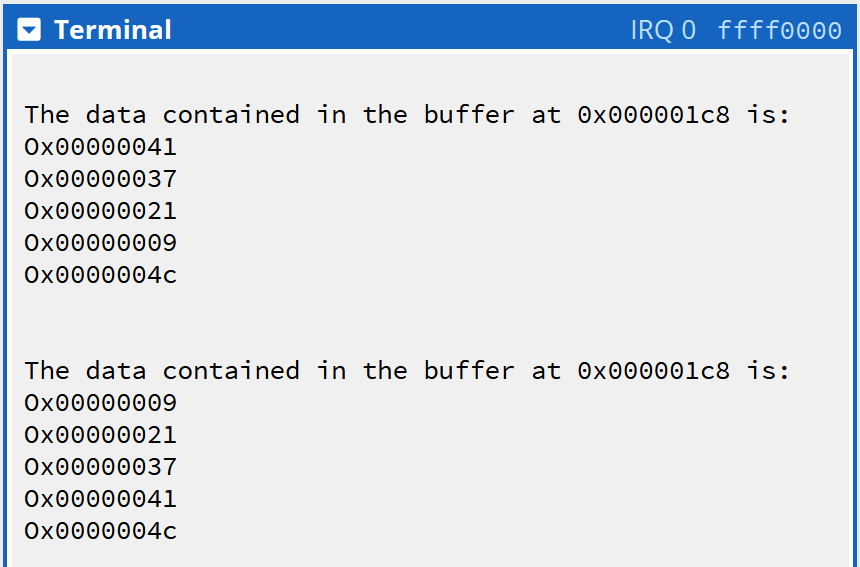
\includegraphics[width=0.7\textwidth]{terminal_output-random_array}
    \caption{
        The output of the bubble sort algorithm written in MIPS given a random unsorted array before
        and after the bubble sort
    }
    \label{fig:out-rand_array}
\end{figure}

\begin{figure}[h!]
    \centering
    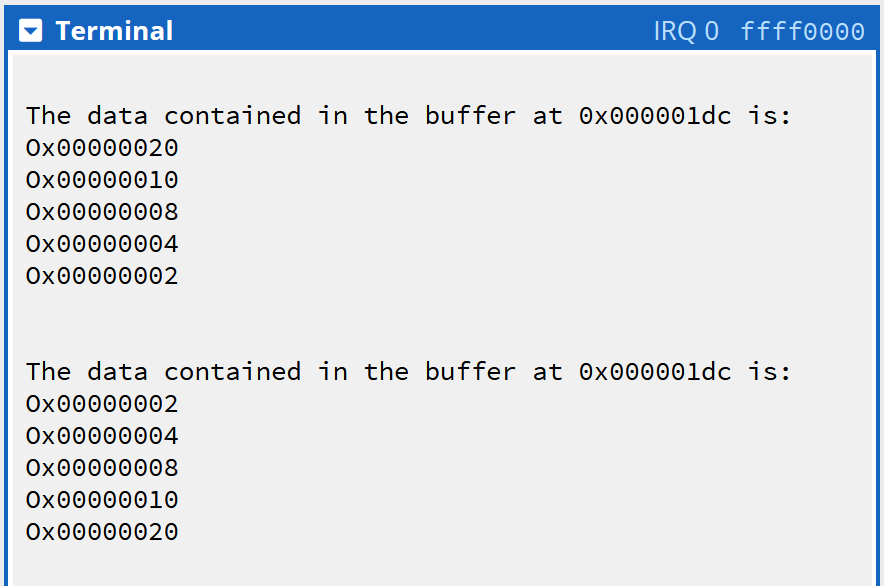
\includegraphics[width=0.7\textwidth]{terminal_output-reverse_sorted_array}
    \caption{
        The output of the bubble sort algorithm written in MIPS given a reverse sorted array before
        and after the bubble sort.
    }
    \label{fig:out-rev_array}
\end{figure}
The bubble sort algorithm works as expected. Figures \ref{fig:out-rand_array} and
\ref{fig:out-rev_array} shows the arrays before and after the running the bubble sort algorithm,
sorting in increasing order. Since the bubble sort displays the correct behavior, the
\verb|compare_and_swap| function works correctly.

\section*{Conclusions}
The \verb|compare_and_swap| function works correctly. The knowledge learned from this lab was
learning how to translate a function from C++ into MIPS assembly as well as correctly providing the
expected arguments and calling the translated function. The skills practiced in this lab was writing
and reading MIPS assembly.


% \newpage
% 
% \section*{References}
% \noindent
% [1]    Computer Organization 22104, EECS, University of Arkansas, “Lab 1,”  Sep. 17, 2024.
% 
% \noindent
% [2]    Computer Organization 22104, EECS, University of Arkansas, “Lab 2,”  Sep. 24, 2024.
% 
% \newpage
% 
% \section*{Appendix}
% \begin{figure}[h!]
%     \centering
%     \includegraphics[width=0.9\textwidth]{foo}
%     \caption{
%         Lorem ipsum dolor sit amet, qui minim labore adipisicing minim sint cillum sint consectetur
%         cupidatat.
%     }
%     \label{fig:foo}
% \end{figure}
% 
% \newpage
% 
% \begin{figure}[h!]
%     \centering
%     \includegraphics[height=0.4\textheight]{bar}
%     \caption{Lorem ipsum something something shorter sentence}
%     \label{fig:bar}
% \end{figure}
\end{document}
